\documentclass[twocolumn, 9pt]{article}

\usepackage[margin=0.8in,bottom=1.25in,columnsep=.4in]{geometry}
\usepackage{amsmath}
\usepackage{amssymb}
\usepackage{listings}
\usepackage{color}
\usepackage{cite}
\usepackage{multicol}
\usepackage{graphicx}

\title{
    50.039 Theory and Practice of Deep Learning\\
    Theory Homework 7
}

\author{Joel Huang 1002530}
\date{\today}

\begin{document}
\maketitle

\section{GRU Equations}
\subsection*{GRU diagram}
\begin{figure}[htbp]
    \centering
    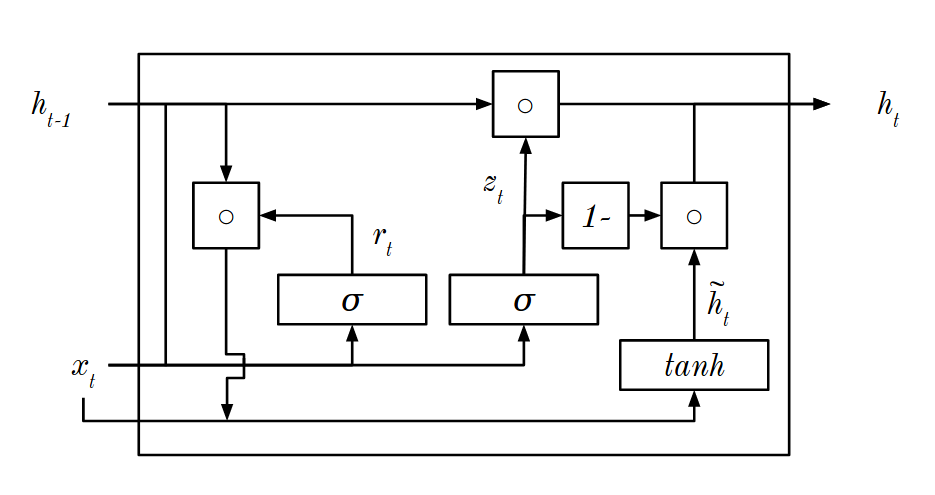
\includegraphics[width=0.95\columnwidth]{gru.png}
    \caption{GRU guts}
    \label{fig:label}
\end{figure}
\subsection*{GRU weight dimensions}
Since we have in the hidden state update, the Hadamard product $z_t \circ h_{t-1}$, and $h_{t-1}: (d_h \times 1)$, then $z_t: (d_h \times 1)$. Its components $W_zx_t$ and $U_xh_{t-1}$ must also have shape $(d_h \times 1)$. If $x_t: (d_x \times 1)$, then:
\begin{equation*}
\begin{split}
    W_z: (d_h \times d_x)\\
    W_r: (d_h \times d_x)\\
    W: (d_h \times d_x)\\
    U_z: (d_h \times d_h)\\
    U_r: (d_h \times d_h)\\
    U_h: (d_h \times d_h)\\
\end{split}
\end{equation*}
\subsection*{Advantage of GRU over LSTM}
GRUs do not have a cell state. Further, LSTMs have separate input and forget gates $i_t$ and $f_t$, while GRUs have a single reset gate $r_t$. Therefore GRUs train with fewer tensor operations and are more computationally efficient than LSTMs.

\section{Defence against adversarial attacks}
The authors of~\cite{ma2018} state that the defensive techniques of adversarial training, distillation, gradient masking, and feature squeezing can generally be evaded by Carlini \& Wagner's optimization-based attacks wholly or partially. They hence use \textit{Local Intrinsic Dimensionality} (LID), to assess the ability of the region surrounding the reference example to fill space.

The idea is that each adversarial example lies in a subspace where all points are also adversarial in a similar way. Recent work has revealed adverserial subspaces to be low-probabiltiy, contiguous multidimensional spaces that are close to the data submanifold, but have class distributions that differ from their closest data submanifold. Density measures thus fail to differentiate an adverserial subspace from the data - instead, LID is used to characterize the adverserial region by revealing samples in the neighborhood of the adversarial sample. In an adversarial subspace, these samples would likely be drawn from more than one manifold, while in a true data manifold, the neighbors would only be drawn from a the same manifold; LID helps to quantify the dimensionality of the space. The deep learning system can then identify adversarial samples using the LID score before rejecting them.

A second way would be to use regular defensive distillation to disable gradient attacks, where a teacher network is first trained at a high temperature to produce classification probabilities $p(x)$ for all samples $x\in X$, then training a secondary network at a high temperature using $p(x)$ as the true labels of $x$; during inference, a low temperature is used, forcing gradients to almost zero and hence numerically unstable.

Since distillation attemps to disable white-box attacks where attackers simply mimic the first model's training scheme, then one way to attack would be to mimic both the first model and second models' training schemes. With knowledge on how many distillations were carried out, and enough computational power, an attacker can simply carry out the same process of distillation and attack the final model in the same way.

\section{Loss functions}
The problem with having an unbounded term in the loss function is that the final objective function (the sum of all component terms) can be minimized by forcing the unbounded term lower and lower, such that any bounded terms need not be minimized in order to minimize the objective function. Capping the unbounded loss term $g_w$ to $\max (g_w, -5-\epsilon)$ ensures that $f_w$ still ``has a chance'' to be minimized when searching for the parameter $w$ that minimizes the objective function, as we can no longer force $g_w$ to be arbitrarily smaller by selection of $w$.

\section{Hierarchical classifiers}
Every level traversed in the tree of classifiers results in a multiplication of the accuracy values of each individual node classifier, reducing the overall accuracy value of the classification task as a whole. For example, for classification task over four classes, a multi-class flat classifier might produce accuracy 0.8. A two-level hierarachical classifier with the same ability can only produce a score of $0.8\cdot0.8$ .

\bibliographystyle{ieeetr}  
\bibliography{references}
\end{document}